\section{Betting, OLO, OCO, Stochastic Optimization, and Model Selection}
\label{sec:appl}

\begin{figure}[t]
\centering
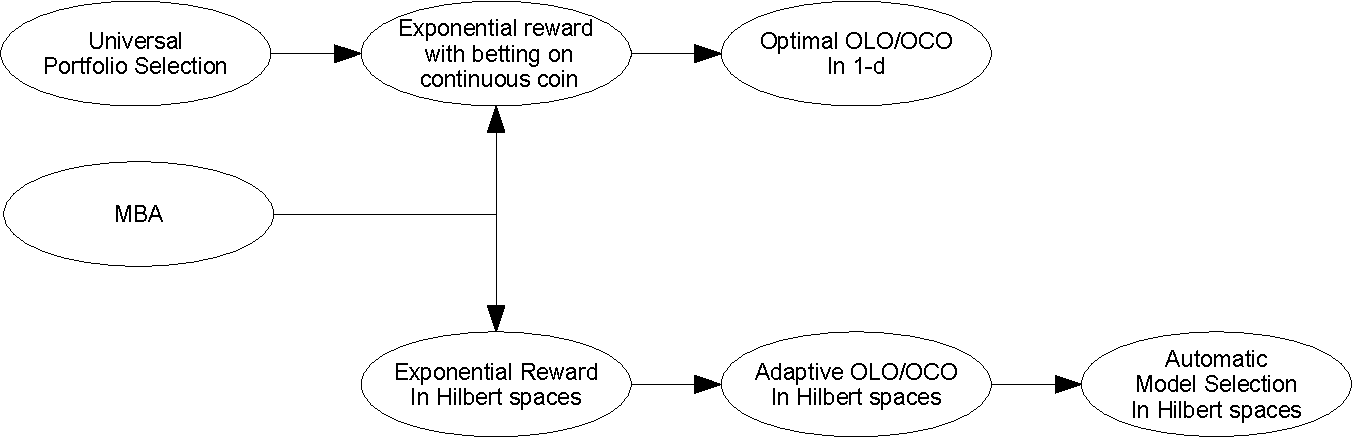
\includegraphics[width=.95\linewidth]{./figs/links_between_areas.pdf}
\caption{The links between the different areas and betting.}
\end{figure}

In this section we will show the connection between portfolio selection, betting on a continous coin, adaptive \ac{OLO}/\ac{OCO}, and automatic model selection. We will prove that, given an ``optimal'' betting algorithm, the same algorithm can be used to solve all the problems listed above.

We will assume that a 1-dimensional algorithm exists, that satisfies the following assumption.
\begin{assumption}
\label{assumption:1-d_algo}
Assume that there exists a sequence of functions $f:\R \times 2^\R \rightarrow \R$ convex in the first argument and an algorithm, that we will denote by \ac{MBA}, that generates $b_t$, where $|b_t|\leq 1$, using in input $x_{t-1} \in \R$, $z_1, \ldots, z_{t-1} \in [-1,1]$, such that
\begin{itemize}
\item $f(0,\{\})=\epsilon>0$;
\item  \begin{equation}
\label{eq:1_d_hp}
(1+b_t z_t) f\left( x_{t-1}^2, \{|z_1|, \ldots, |z_{t-1}|\} \right) \geq f\left( (x_{t-1}+z_t)^2, \{|z_1|, \ldots, |z_t|\}\right), \ \ \forall z_{t} \in [-1,1]~.
\end{equation}
\end{itemize}
\end{assumption}

By induction is easy to prove that such algorithm can indeed be used as a betting algorithm. 
\begin{theorem}
\label{theo:1-d_reward}
Assume that Assumption \ref{assumption:1-d_algo} holds and use the \ac{MBA} with $x_{t-1}=|\sum_{i=1}^{t-1} g_i|$ and $z_t=g_t$.
Then, for any sequence of outcomes $g_t \in [-1,1]$, the following holds
\[
\wealth_n = \epsilon+\sum_{t=1}^n g_t w_t \geq f\left( \left(\sum_{i=1}^{t-1} g_i \right)^2, \left\{|z_1|, \ldots, |z_n|\right\}\right)~.
\]
\end{theorem}

Even more importantly, the \ac{MBA} can also be used to prove lower bound on the reward in Hilbert Spaces.
%\noindent\textbf{From 1-dimension to Hilbert spaces.}
\begin{theorem}
\label{theo:hilbert_reward}
  Assume that \ref{assumption:1-d_algo} holds.
  Let $\bg_t \in \fH$ an arbitrary sequence of vector, such that $\norm{\bg_t} \leq 1$ and define the vector $\btheta_t=\sum_{i=1}^{t} \bg_i$.
  Use the Algorithm in \ref{assumption:1-d_algo} with the sequence $x_{t-1}= \norm{\btheta_{t-1}}$.
  Define a vectorial algorithm that at each step outputs $\bw_t = b_t \frac{\btheta_{t-1}}{\norm{\btheta_{t-1}}} \wealth_{t-1}$. Then the following holds
  \[
  \wealth_{n} = \epsilon + \sum_{t=1}^n \langle \bg_t, \bw_t \rangle \geq f\left( \norm{\sum_{t=1}^n \bg_t}^2, \left\{\norm{\bg_1}, \ldots, \norm{\bg_n}\right\}\right)~.
  \]
\end{theorem}
This theorem is useful to prove regret bounds in Hilbert spaces, as shown in the next part.

\vspace{0.2cm}\noindent\textbf{From Reward to Regret.}
The reward and regret view on online learning are equivalent: an algorithm guarantees low regret iff it guarantees high reward. The following Theorem makes this claim rigorous. Notice that the algorithm is exactly the same in the two setting.
\begin{theorem}[\citet{McMahanO14}]
  \label{thm:rrdual}
  Let $\Psi:\mathcal{H} \rightarrow (-\infty, +\infty]$ be a lower semicontinuos and convex function, with $dom \Psi \neq \emptyset$. An
  algorithm for the player guarantees
  \[
  \gain_n \geq \Psi\left(\sum_{t=1}^n \bg_t\right) - \epsilon \quad \quad \quad \textnormal{ for any } \bg_1, \dots, \bg_n
  \]
  for a constant $\epsilon \in \R$ if and only if it
  guarantees
  \begin{equation}\label{eq:regb}
  \qquad Regret_n(\bu) \leq \Psi^*(\bu) + \epsilon \quad \quad \quad \textnormal{ for all } \bu \in \fH \textnormal{ and } \bg_t \in \fH, \forall 1\leq t\leq n~.
  \end{equation}
\end{theorem}
So, a betting algorithm can be used for online learning and vice-versa. However, as it was already stressed in \citet{McMahanO14}, the reward view has the big advantage of having one variable less, the competitor $\bu$.
Moreover, as we will show in Section~\ref{sec:algo}, designing and analysing algorithms in one of the two views could be much easier than in the other one.
Coupling Theorem~\ref{thm:rrdual} with Theorem~\ref{theo:hilbert_reward}, we have the following Corollary.
\begin{cor}
\label{theo:hilbert_regret}
Assume that \ref{assumption:1-d_algo} holds. Then there exists a reduction of the \ac{MBA} that produces a sequence of vectors $\bw_t$ that satisfy
\[
Regret_n(\bu) \leq f^*\left( \norm{\sum_{t=1}^{n} \bg_t}^2, \left\{\norm{\bg_1}, \ldots, \norm{\bg_n}\right\}\right)+\epsilon \quad \quad \quad \textnormal{ for all } \bu \in \fH \textnormal{ and } \bg_t \in \fH, \forall 1\leq t\leq n,
\]
where the conjugation is taken w.r.t. the first argument of $f$.
\end{cor}

\vspace{0.2cm}\noindent\textbf{\ac{OLO}, \ac{OCO} and Stochastic Convex Optimization.}
From the property of the sub-gradient of a convex function we have that, for any sequence of convex functions $f_1, \ldots, f_n$, vectors $\bw_1,\ldots, \bw_n$, and $\bg_t \in f_t(\bw_t)$, we have
\[
Regret^{OCO}_n(\bu) = \sum_{t=1}^n \left( f_t(\bw_t) -f_t(\bu)\right) \leq \sum_{t=1}^n \langle \bw_t-\bu, \bg_t\rangle = Regret_n(\bu)~.
\]
Hence, the regret w.r.t. to arbitrary convex functions is upper bounded by linear regret. This means that an \ac{OLO} algorithm can be used to solve an \ac{OCO} problem, just feeding the algorithm with loss vectors $g_t$ equal to the subgradients of the functions $f_t$.

Also, a regret bound can be transformed into a convergence guarantee for optimization of convex functions.
In particular, we have the following Theorem from~\citet{Cesa-BianchiCG04}.
%
\begin{theorem}
\label{theo:online_to_batch}
Let $\bw_1, \cdots, \bw_n \in \fH$ the vector produced by an OLO algorithm with a regret guarantee $Regret_n(\bu)$.
Let $F:\fH\rightarrow\R$ a convex function, and fix the vectors $\bg_t$ to be unbiased estimate of the gradient of $F$ in $\bw_t$. Then, the following holds
\[
\E\left[F\left(\frac{1}{n} \bw_t\right)\right] \leq \frac{\E[Regret_n(\bu)]}{n}~.
\]
\end{theorem}

High probability bounds can be also easily obtained, assuming more on the function $F$~\citep{Cesa-BianchiCG04}.
The above theorem says that, if the regret grows, for example, as $\scO(\sqrt{n})$, the OLO algorithm can be used as a stochastic optimization algorithm with convergence in expectation $\scO(\frac{1}{\sqrt{n}})$.


\vspace{0.2cm}\noindent\textbf{Adaptive Algorithms for OLO and Self-tuning Model Selection.}
In learning theory a key concept is the one of regularization. If the concept class we are learning is too rich, we need to constrain the complexity of the trained predictor. A regularizer is achieving this, biasing the classifieres towards a small region of the space. However, it is known that the optimal amount of regularization is completely problem-dependent. Hence, the regularizer becomes another parameter to be learned.

Most, if not all, the machine learning algorithms uses a two-stages process to find the optimal amount of regularization. First, the algorithm is trained with a fixed regularization parameter. Second, its generalization performance is estimated together with a change in the regularization parameter. These two steps are repeated till convergence.

Surprisingly enough, \citep{Orabona14} proved that, when the regularizer is the squared norm of the Hilbert space, the above lenghty procedure can be avoided with a stochastic learner.
In particular, instead of solving a series of regularized ERM problems, with different amounts of regularization, one can use a simple prarameter-free stochastic gradient descent procedure over the training samples and achieve the same performance.
More rigorously, the follwing theorem holds.
\begin{theorem}
\label{theo:self_tune}
Assume that there is an online algorithm whose $Regret_n(\bu)$ is $\scO\left(\norm{\bu}\sqrt{n} (\ln(n))^\alpha\right)$. Then the following holds
\begin{equation}
\label{eq:self_tune}
\E\left[\RiskLoss\left(\frac{1}{T} \sum_{t=1}^n \bw_t\right)\right] \leq \scO\left(\inf_{\bu} \min_{\lambda>0} \RiskLoss(\bu) + \lambda \norm{\bu}^2 +\frac{(\ln(n))^{2 \alpha}}{\lambda \, n} \right)~.
\end{equation}
% Let $\bw_1, \cdots, \bw_n \in \fH$ the vector produced by the PiSTOL algorithm.
% Let $\ell:\R\rightarrow\R$ a convex and Lipschitz function, and fix the vectors $\bg_t$ to be unbiased estimate of the gradient of $F$ in $\bw_t$. Then, the rate of convergence of $\E\left[Risk_F\left(\frac{1}{n} \bw_t\right)\right]$ is the same of regularized ERM algorithm with the (unknown) optimal amount of regularization.
\end{theorem}
To better appreciate this bound, it is useful to compare it with a generalization bound you get from a regularized \ac{ERM} solution, e.g. the one in \citet{SridharanSSS09}.
There, they prove that, with probability at least $1-\delta$, we have
\begin{equation}
\label{eq:fast_rate_srebro}
\RiskLoss\left(\hat{\bw}\right) \leq \scO\left(\inf_{\bu} \RiskLoss(\bu) + \lambda \norm{\bu}^2 +\frac{\ln \frac{1}{\delta}}{\lambda \, n} \right),
\end{equation}
where 
\begin{align*}
\hat{\bw}=\argmin_{\bw} \frac{\lambda}{2}\norm{\bw}^2 + \sum_{t=1}^n f_t(\bw_t)~.
\end{align*}
Ignoring the fact that the bound in Theorem~\ref{theo:self_tune} is only in expectation, the bound in \eqref{eq:fast_rate_srebro} is missing the minimum over $\lambda$, that is present in \eqref{eq:self_tune}. Hence, to obtain the optimal performance in the regularized \ac{ERM} setting we have to prove different values of $\lambda$, while in Theorem~\ref{theo:self_tune} the tuning is automatic. This is particular important in infinite dimensional Hilbert spaces, where the infimum could not be attained by a vector in the space~\cite{Orabona14}.

The only missing piece is to prove that the existence of the \ac{MBA} guarantees to have an algorithm that satisfies the regret guarantee in the hypothesis of Theorem~\ref{theo:self_tune}. Indeed, we have the following Theorem.
\begin{theorem}
\label{theo:regret_pistol}
Assume that \ref{assumption:1-d_algo} holds and there exist constants $A,B,C,D\geq0$ independent from $t$ such that the function $f(x,\{z_1, \ldots, z_t\}) \geq B t^{-C} \exp(\frac{x}{A t})-D$.
Then there exists an algorithm, that uses the \ac{MBA} as a subroutine, that guarantees $Regret_n(\bu)=\scO\left(\norm{\bu}\sqrt{n \ln(n \norm{\bu}+1)}\right)$.
\end{theorem}

%In reality, the connection between betting and self-tuning regularized ERM is actually stronger. In fact, the following theorem can be proved.
%\begin{theorem}
%If a betting strategy against a coin with outcomes in $[-1,1]$ guarantees an exponential reward, the same algorith used for SGD over the risk of a convex loss will guarantee optimal rate of convergence to the Bayes risk.
%\end{theorem}


To summarize, the existence of a simple 1-d algorithm guarantees, though a straighforward reduction, the possibility of learning in Hilbert spaces, in the online setting and stochastic setting. Moreover, if the algorithm guarantees an exponential growth of the wealth, a reduction allows to use it for obtain optimal rates of convergence to best risk in a function class, without having to choose the regularization parameter.
In the next section we will explain what are the difficulties in designing such 1-d algorithm and in Section~\ref{sec:algo} we will present our solution.